\section{Trigonometric Functions}

\subsection{Definition and Projections}

A {\bf trigonometric function}, by definition, is any function of an angle.  However, when one says "trigonometric functions", it is universally understood that one is referring to a specific function known as the {\bf sine}, and its related functions.  These functions are derived from the projection of an angle into a {\bf Cartesean coordinate system}.  A {\bf projection}, for our purposes, can be thought of as the 'shadow' that one line casts on another.  Note that the shadow's edge is at a right angle to the line being shadowed; this is important.\\

\begin{figure}[htb]
\center
\caption{A projection of $r$ onto $x$.}
\label{fig:projection}
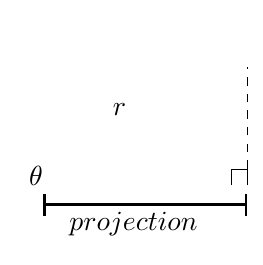
\begin{tikzpicture}[inner sep=0pt,minimum size=0mm]
\node () at (0,2){};
\node () at (1.325,-0.5) {$projection$};
\node () at (40:1.5) {$r$};

\LANGLE{0,0}{3}{0}{30}{$\theta$}
\XAXIS{1}{0}{2.5}

\draw[|-|,line width=1pt] (0,-0.25) -- (1.5*1.732,-0.25);

\draw[dashed] (1.5*1.732,0) -- (1.5*1.732,1.5);
\draw (1.5*1.732-0.2,0) -- (1.5*1.732-0.2,0.2) -- (1.5*1.732,0.2) -- (1.5*1.732,0.0);

\end{tikzpicture}
\end{figure}


\subsection{Sine et al.}

So, let's take a line segment of length $r$ and rotate it by angle $\theta$, and let $y$ be the length of the projection of this line segment onto the y axis of our coordinate system.\\

\begin{figure}[htb]
\center
\caption{A projection of $r$ onto the x and y axes.}
\label{fig:projection_onto_axes}
\begin{tikzpicture}[inner sep=0pt,minimum size=0mm]
\node () at (0,2.5){};
\node () at (1.325,-0.85) {$x$};
\node () at (-0.85,0.75) {$y$};

\node () at (40:1.5) {$r$};

\LANGLE{0,0}{3}{0}{30}{$\theta$}
\PAXES{0}{0}{3}{1.7}

\draw[|-|,line width=1pt] (-0.5,0) -- (-0.5,1.5);
\draw[|-|,line width=1pt] (0,-0.5) -- (1.5*1.732,-0.5);
\draw[dashed] (1.5*1.732,1.5) -- (0,1.5);
\draw (0,1.5-0.2) -- (0.2,1.5-0.2) -- (0.2,1.5) -- (0,1.5);
\draw[dashed] (1.5*1.732,0) -- (1.5*1.732,1.5);
\draw (1.5*1.732-0.2,0) -- (1.5*1.732-0.2,0.2) -- (1.5*1.732,0.2) -- (1.5*1.732,0.0);

\end{tikzpicture}
\end{figure}

$y$ must be some function of the line segment's length, and the angle of rotation, $r$ and $\theta$.  By using similar triangles, we can show that $y$ is directly proportional to $r$, meaning that $y = rf(\theta)$, the length multiplied by some unknown function of the angle.  This function $f(\theta)$ is of interest, so we rearrange the equation to isolate it.\\

\tab$y = rf(\theta)$ \ \  \implies  \ \  $f(\theta)=\frac{y}{r}$\\

So, $f(\theta)$ is the ratio of the length of the line segment to its projection on the y axis.  This function is a special trigonometric function called the {\bf sine} of an angle. \\

\tab $f(\theta) = sin(\theta) = \frac{y}{r}$, \ \ $y = r \ sin(\theta)$ \ \ \ (remember these!)\\

The {\bf cosine} of an angle is a similiar function, but uses the projection onto the x axis instead of the y axis.\\

\tab $cos(\theta) = \frac{x}{r}$, \ \ $x = r \ cos(\theta)$ \\

Another useful function is the {\bf tangent} of an angle, which is the sine divided by the cosine.\\

\tab$tan(\theta)=\frac{sin(\theta)}{cos(\theta)} = \frac{y}{r}/\frac{x}{r} = \frac{y}{x}$\\

These three functions are the basic trigonometric functions.  However, there are three other functions, each of which is the {\bf reciprocal}, or multiplicative inverse, of a basic trigonometric function.\\

The {\bf secant} of an angle is the reciprocal of the cosine.\\

\tab$sec(\theta) = \frac{1}{cos(\theta)} = \frac{r}{x}$\\

The {\bf cosecant} of an angle is the reciprocal of the sine.\\

\tab$csc(\theta) = \frac{1}{sin(\theta)} = \frac{r}{y}$\\

The {\bf cotangent} of an angle is the reciprocal of the tangent.\\

\tab$cot(\theta) = \frac{1}{tan(\theta)} = \frac{x}{y}$\\

\newpage

\subsection{Right Triangles}
A more common visual interpretation of trigonometric functions is created by using the sides of a right triangle.  The sides of this right triangle, due to the properties of parallel lines, are equal in size to the x and y projections of $r$, thus sine and cosine are also the ratio of the sides of this triangle.\\

\begin{figure}[htb]
\center
\caption{A right triangle from projections.}
\label{fig:right_triangle_projections}
\begin{tikzpicture}[inner sep=0pt,minimum size=0mm]
\node () at (0,2){};
\node () at (1.325,-0.85) {$x$};
\node () at (3.85,0.75) {$y$};
\node () at (0.75,0.2) {$\theta$};

\node () at (40:1.5) {$r$};

\LANGLE{0,0}{3}{0}{30}{}

\draw[|-|,line width=1pt] (3.65,0) -- (3.65,1.5);
\draw[|-|,line width=1pt] (0,-0.5) -- (1.5*1.732,-0.5);
\draw[dashed] (1.5*1.732,0) -- (1.5*1.732,1.5);
\draw (1.5*1.732-0.2,0) -- (1.5*1.732-0.2,0.2) -- (1.5*1.732,0.2) -- (1.5*1.732,0.0);

\end{tikzpicture}
\end{figure}

From this, we can again derive the trigonometric functions.\\

\tab$sin(\theta) = \frac{y}{r}$ \ \ \ \ $csc(\theta) = \frac{r}{y}$\\

\tab$cos(\theta) = \frac{x}{r}$ \ \ \ \ $sec(\theta) = \frac{r}{x}$\\

\tab$tan(\theta) = \frac{y}{x}$ \ \ \ \ $cot(\theta) = \frac{x}{y}$\\

\newpage
\subsection{Review}

\begin{enumerate}

\item{What is the definition of a trigonometric function?}

\item{What is the definition of a projection?}

\item{What is the definition of sine?  of cosine?}

\item{Which axis is the sine projected on?  The cosine?  Don't forget this!}

\item{Draw an angle and its projections, then define the sine and cosine of that angle.}

\item{What is the definition of tangent?  of secant?  of cosecant?  of cotangent?}

\item{Is secant the reciprocal of sine or cosine?  Don't forget this!}

\item{Why can you also use a right triangle to define sine and cosine?}

\item{Draw a right triangle, and write the length of the sides in terms of one angle and the length of the hypotenuse.}

\item{From the previous question, how do you know which side corresponds with sine, and which with cosine?}

\end{enumerate}

